\section{Background}

This paper takes the API and load balancers designed in
Mantle~\cite{sevilla:sc15-mantle}, the programmabile file system metadata load
balancer for Ceph, and applies them to
HXHIM~\cite{greenberg:hotstorage2015-mdhim}, the distributed key-value store
designed for HPC.

\subsection{ParSplice}
\label{sec:parsplice}

\begin{figure}[t]
  \noindent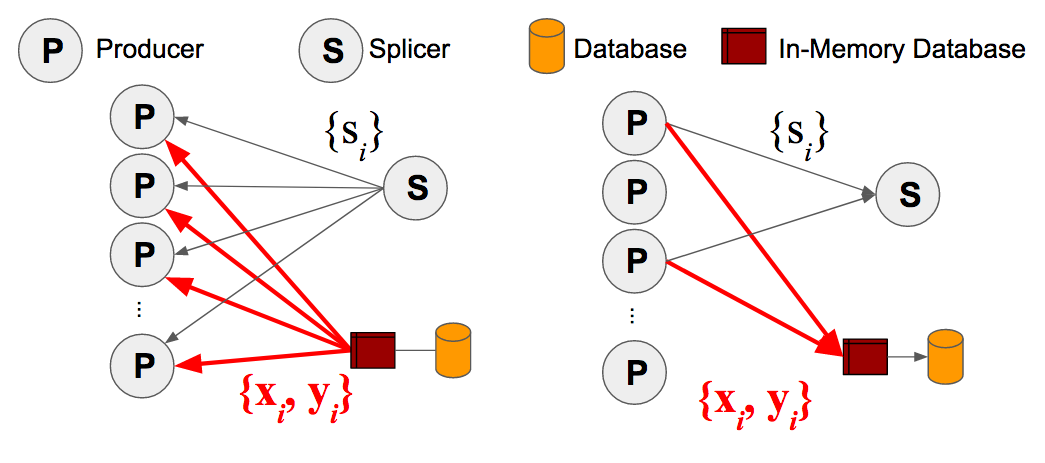
\includegraphics[width=19pc,angle=0]{figures/arch-parsplice.png}\\
  \caption{ParSplice is a ready-heavy HPC application where producers use a
  database for consistency. Replacing the single-node database with HXHIM
  improves performance with load balancing.
  \label{fig:arch-parsplice}}
\end{figure}

It has 4 phases:

\begin{enumerate}

  \item splicer (S) tells producers (P) to compute segments for state \(s_i\)

  \item P`s pull initial coordinates \{\(x_i, y_i\)\} from database

  \item a P inserts completed coordinates for segment \(s_i\) into database and
  S broadcasts next segment(s) \(s_j\) 

  \item P`s pull new segment coordinates \{\(x_j, y_j\)\}
\end{enumerate}



\subsection{Mantle: File System Metadata Load Balancer}
\label{sec:mantle}

% What is Mantle?
Mantle is an API that lets admnistrators control file system metadata load
balancing. Mantle speeds up file systems by making metadata access faster,
leveraging the fact that file system metadata IO imposes small and frequent
accesses on the underlying storage system. Since data IO does not scale like
metadata IO~\cite{roselli:atec2000-FS-workloads}, finding optimal ways to
measure, migrate, and partition metadata load is a relatively new field, but
has been shown to lead to large performance increases and more scalable file
systems~\cite{zheng:pdsw2014-batchfs, grider:pdsw2015-marfs,
ren:sc2014-indexfs, patil:fast2011-giga+, brandt:msst2003-lh}.  Mantle can use
strategies from these papers to control how to distribute or concentrate file
system metadata.

% How does it work?
It was built on CephFS, the file system above Ceph, so it inherits many of
characteristics of the CephFS architecture, like the dedicated metadata cluster
and heartbeat mechanisms shown at the top of Figure~\ref{fig:arch-mantle}.
Each metadata server manages differently sized subtrees of the logical
namespace and migration decisions are made synchronously, every 10 seconds.
CephFS already had the mechanisms for load balancing, namely the ability to
measure the load on a subtree, to migrate subtrees, and to partition subtrees
into smaller subtrees, but it had hard-coded, ad-hoc policies for guiding the
migrations.  Mantle reads user-defined policies written in Lua and returns
decisions for how load should be migrated given the state of the cluster and
the behavior of the workload. The hooks in Figure~\ref{fig:arch-mantle} show
where CephFS calls out to the Mantle library to make decisions. While the
decisions were made by Mantle, CephFS used its internal mechanisms to do the
load balancing.

% The actual policies
The Mantle paper implemented three balancers and tested them under
metadata-intensive workloads. The Greedy Spill balancer, which was based
on~\cite{patil:fast2011-giga+}, sheds have its load aggressively when there are
avaiable servers. Part of the Lua code for implementing this balancer is shown
in~\ref{fig:arch-mantle-example}.  The Fill and Spill balancer, which was based
on~\cite{pai:asplos1998-lard} sheds a fraction of the load only when the server
is overloaded. Finally, the Adaptable balancer, which was based
on~\cite{weil:sc2004-dyn-metadata, weil:osdi2006-ceph}, sheds a fraction of the
load frequently.

% What is the status?
It was merged\footnote{https://github.com/ceph/ceph/pull/5155} and is starting
to get users who are frustrated with the hard-coded load balancing policies
that are shipped with CephFS. It was re-implemented using the ``programmable
storage" approach~\cite{sevilla:eurosys17} to reduce lines of code for doing
things like versioning and distributing balancer version.  Although Mantle is
heavily integrated the daemons that compose an Ceph cluster, using Ceph's
naming conventions and internal libraries like Ceph's version of protocol
buffers, there is no reason that it cannot be extracted.

\begin{figure}[tb]
  \noindent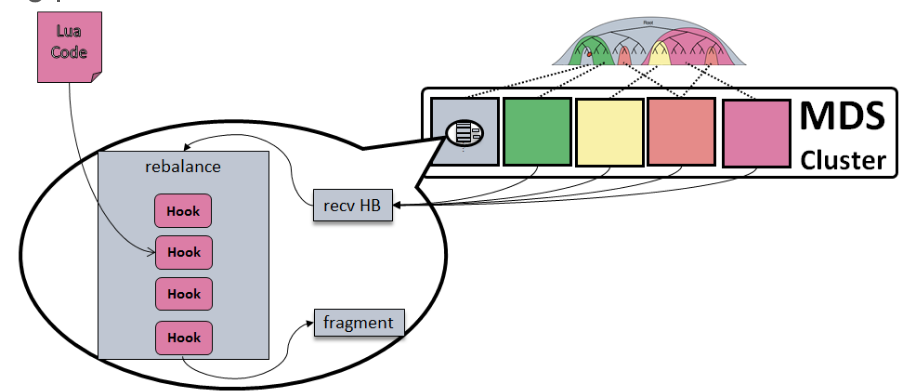
\includegraphics[width=19pc,angle=0]{figures/arch-mantle.png}\\
  \caption{The Mantle API lets adminstrators control load balancing by
  changing the poicies for how to distribution or concentrate file system
  metadata. It was merged into CephFS and inherits many aspects of that
  architecture. Although it has the load balancing structure and logic from
  CephFS (gray boxes), the actual API is not dependent on that code base.}
  \label{fig:arch-mantle}
\end{figure}
\begin{figure}[tb]
  \noindent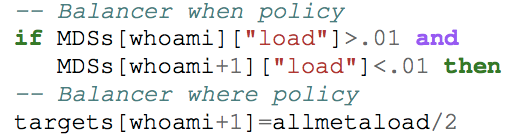
\includegraphics[width=19pc,angle=0]{figures/arch-mantle-example.png}\\
  \caption{The Greedy Spill balancer written in Lua using the Mantle API.}
  \label{fig:arch-mantle-example}
\end{figure}

\subsection{HXHIM: Key-Value Store for HPC}
\label{sec:hxhim}

\begin{figure}[tb]
  \noindent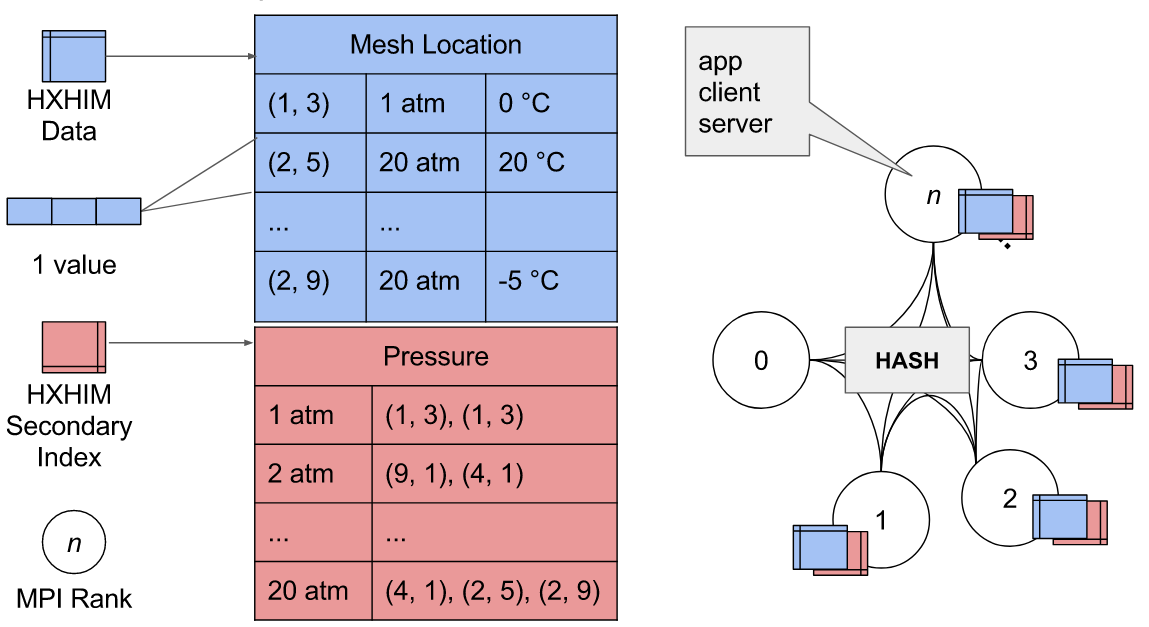
\includegraphics[width=19pc,angle=0]{figures/arch-hxhim.png}\\
  \caption{The HXHIM architecture.}
  \label{fig:arch-hxhim}
\end{figure}

% What is HXHIM
HXHIM is a key-value store designed for HPC architectures and multi-dimensional
data. It is based off MDHIM~\cite{greenberg:hotstorage2015-mdhim}, the
multi-dimensional indexing middleware. Figure~\ref{fig:arch-hxhim} has a crude
sketch of the HXHIM architecture. Each MPI rank has an instance of the
application, which has the client library linked in. An MPI rank can also have
a ``range server", which stores the key-value pairs in a local databse (either
LevelDB or MySQL). Data is located with a consistent hash, which is
configurable.

% What are the indexes?
The primary and secondary indices shown on the right side of
Figure~\ref{fig:arch-hxhim} are views of the data that the range server
manages.  The primary index is the same hash used by the global partitioner.
The secondary index or indices are user-defined tables organized in a different
way from the primary index. The goal of the secondary indices is to speed up
queries that need to aggregate dat ({\it e.g.} find the maximum values). In the
example, the range server and the key in the primary index is located with a
hash of the mesh location. The secondary index is organized by pressure, so
queries asking for a certain atmosphere can be serviced in O\(1\), consisting
of one lookup in the pressure index and one lookup into the primary index.

% Why is it tailored to HPC?
HXHIM tailors its mechanisms and policies to HPC, showing improved performance
over cloud-based key-value stores like Cassandra. It has cursor types for
walking the key-value store, bulk operations for exploiting data locality,
per-job server spawning, and pluggable backends for its local database and
network type (infiniband/RDMA). Its policies are flexible, supporting
customized partitioning strategies and user-defined secondary indices. This
allows the system to choose whether to send load to the client or server.

\subsection{Comparing Mantle and HXHIM}
\begin{figure}[tb]
  \noindent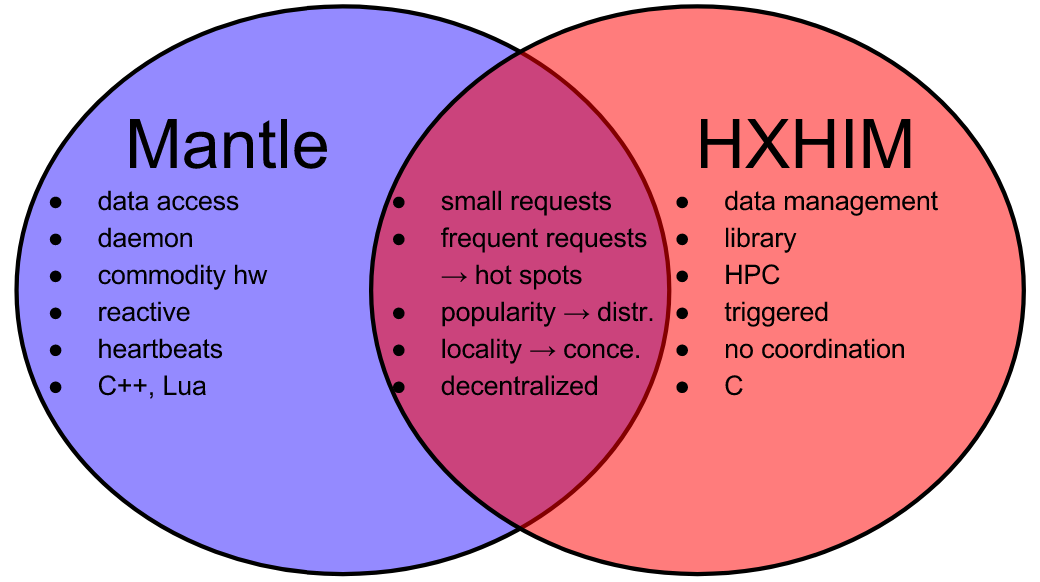
\includegraphics[width=19pc,angle=0]{figures/arch-comparison.png}\\
  \caption{Comparing the design goals and implementations of Mantle and HXHIM.}
  \label{fig:arch-comparison}
\end{figure}

% Why are the designed for the same type of workload?
The intersecting portions of Figure~\ref{arch-comparison} shows how Mantle and
HXHIM have similar designs. The workloads are very similar as the the services
respond to small and frequent requests, which results in hot spots and flash
crowds. As a result, popularity of the data, not the size, drives distribution
in both systems. Both workloads also have data locality so the systems have
mechanisms for leveraging requests with similar semantic meaning. Finally, the
overall design of both systems is decentralized meaning that there is no
centralized scheduler and each server has an inconsistent global view.

% What are the challenges?
Despite the similarities, integrating the Mantle API with HXHIM has both design
and technical challenges. Mantle is reactive to the workload as opposed to
HXHIM migrations, which are triggered based on the request type. As a result,
Mantle has functionality for exchanging server 
utilization (CPU, network, memory) and workload (tracks request types). HXHIM 
% RESUME


